Målet med brukbarhetstesten er å finne områder der brukeren ikke forstår hvordan
han skal komme seg videre i programflyten, og se at brukeren klarer å finne
den informasjonen han ønsker.

Etter testen ga vi dem et SUS-skjema - System Usability Scale. Dette lar
brukeren gi tilbakemelding i form av poeng fra 1-5 på skalaen sterkt enig til
sterkt uenig. Testen er delt opp i likt antall negativt og positivt ladde
spørsmål. Disse spørsmålene er vevd sammen annenhver, men i teksten nedenfor
kaller jeg positive spørsmål del1 og negative del2 siden disse summeres hver for
seg. Del1 = spørsmål 1,3,5,7 og 9 og del2 = 2,4,6,8,10.

Hos Merete scoret vi 4+3+4+4+2 = 17 på del1 og 2+3+1+3+4 = 13 på
del2. Hos Ove scoret vi 3+2+3+3+3 = 14 på del1 og 4+4+3+3+4 = 18 på
del2. Dette ga score (17+13) * 2.5 = 75 for Merete og (14+18) * 2.5 = 80
fra Ove. De to scorene ble altså 75/100 fra Merete og 80/100 fra Ove. Dette gir
et snitt på 77.5/100.

Det er litt interessant og observere at Merete ga høyest poeng på de positivt
ladde spørsmålene, mens Ove ga mest poeng på de negativt ladde spørsmålene.

Mye av den tilbakemeldingen vi fikk etter testen tydet på at det som var mest
uklart var flyten gjennom de forskjellige casene. Det var litt forvirrende når
både case 4 og 5 var avhengige av at case 1 og 2 ble gjort om igjen. Vi burde
nok ha fokusert på å lage mer frittstående caser, slik at vi bedre kunne testet
flyten i programmet, og ikke i casene.

En score på 77.5 er ikke spesielt bra, men jeg tror en del av minuspoengene kom
fra litt forvirrende scenarier, og at de hadde litt høyere forventninger når
papirprotypene våre var interaktive og på pcen. I forhold til den gruppen som
vi testet sammen med, så var det morsomt når de la frem masse informasjon i
et klikk, mens når vi la inn masse informasjon når en hoppet til neste bilde, så
virket det kanskje litt forvirrende.

\begin{figure}[obs]
\centering
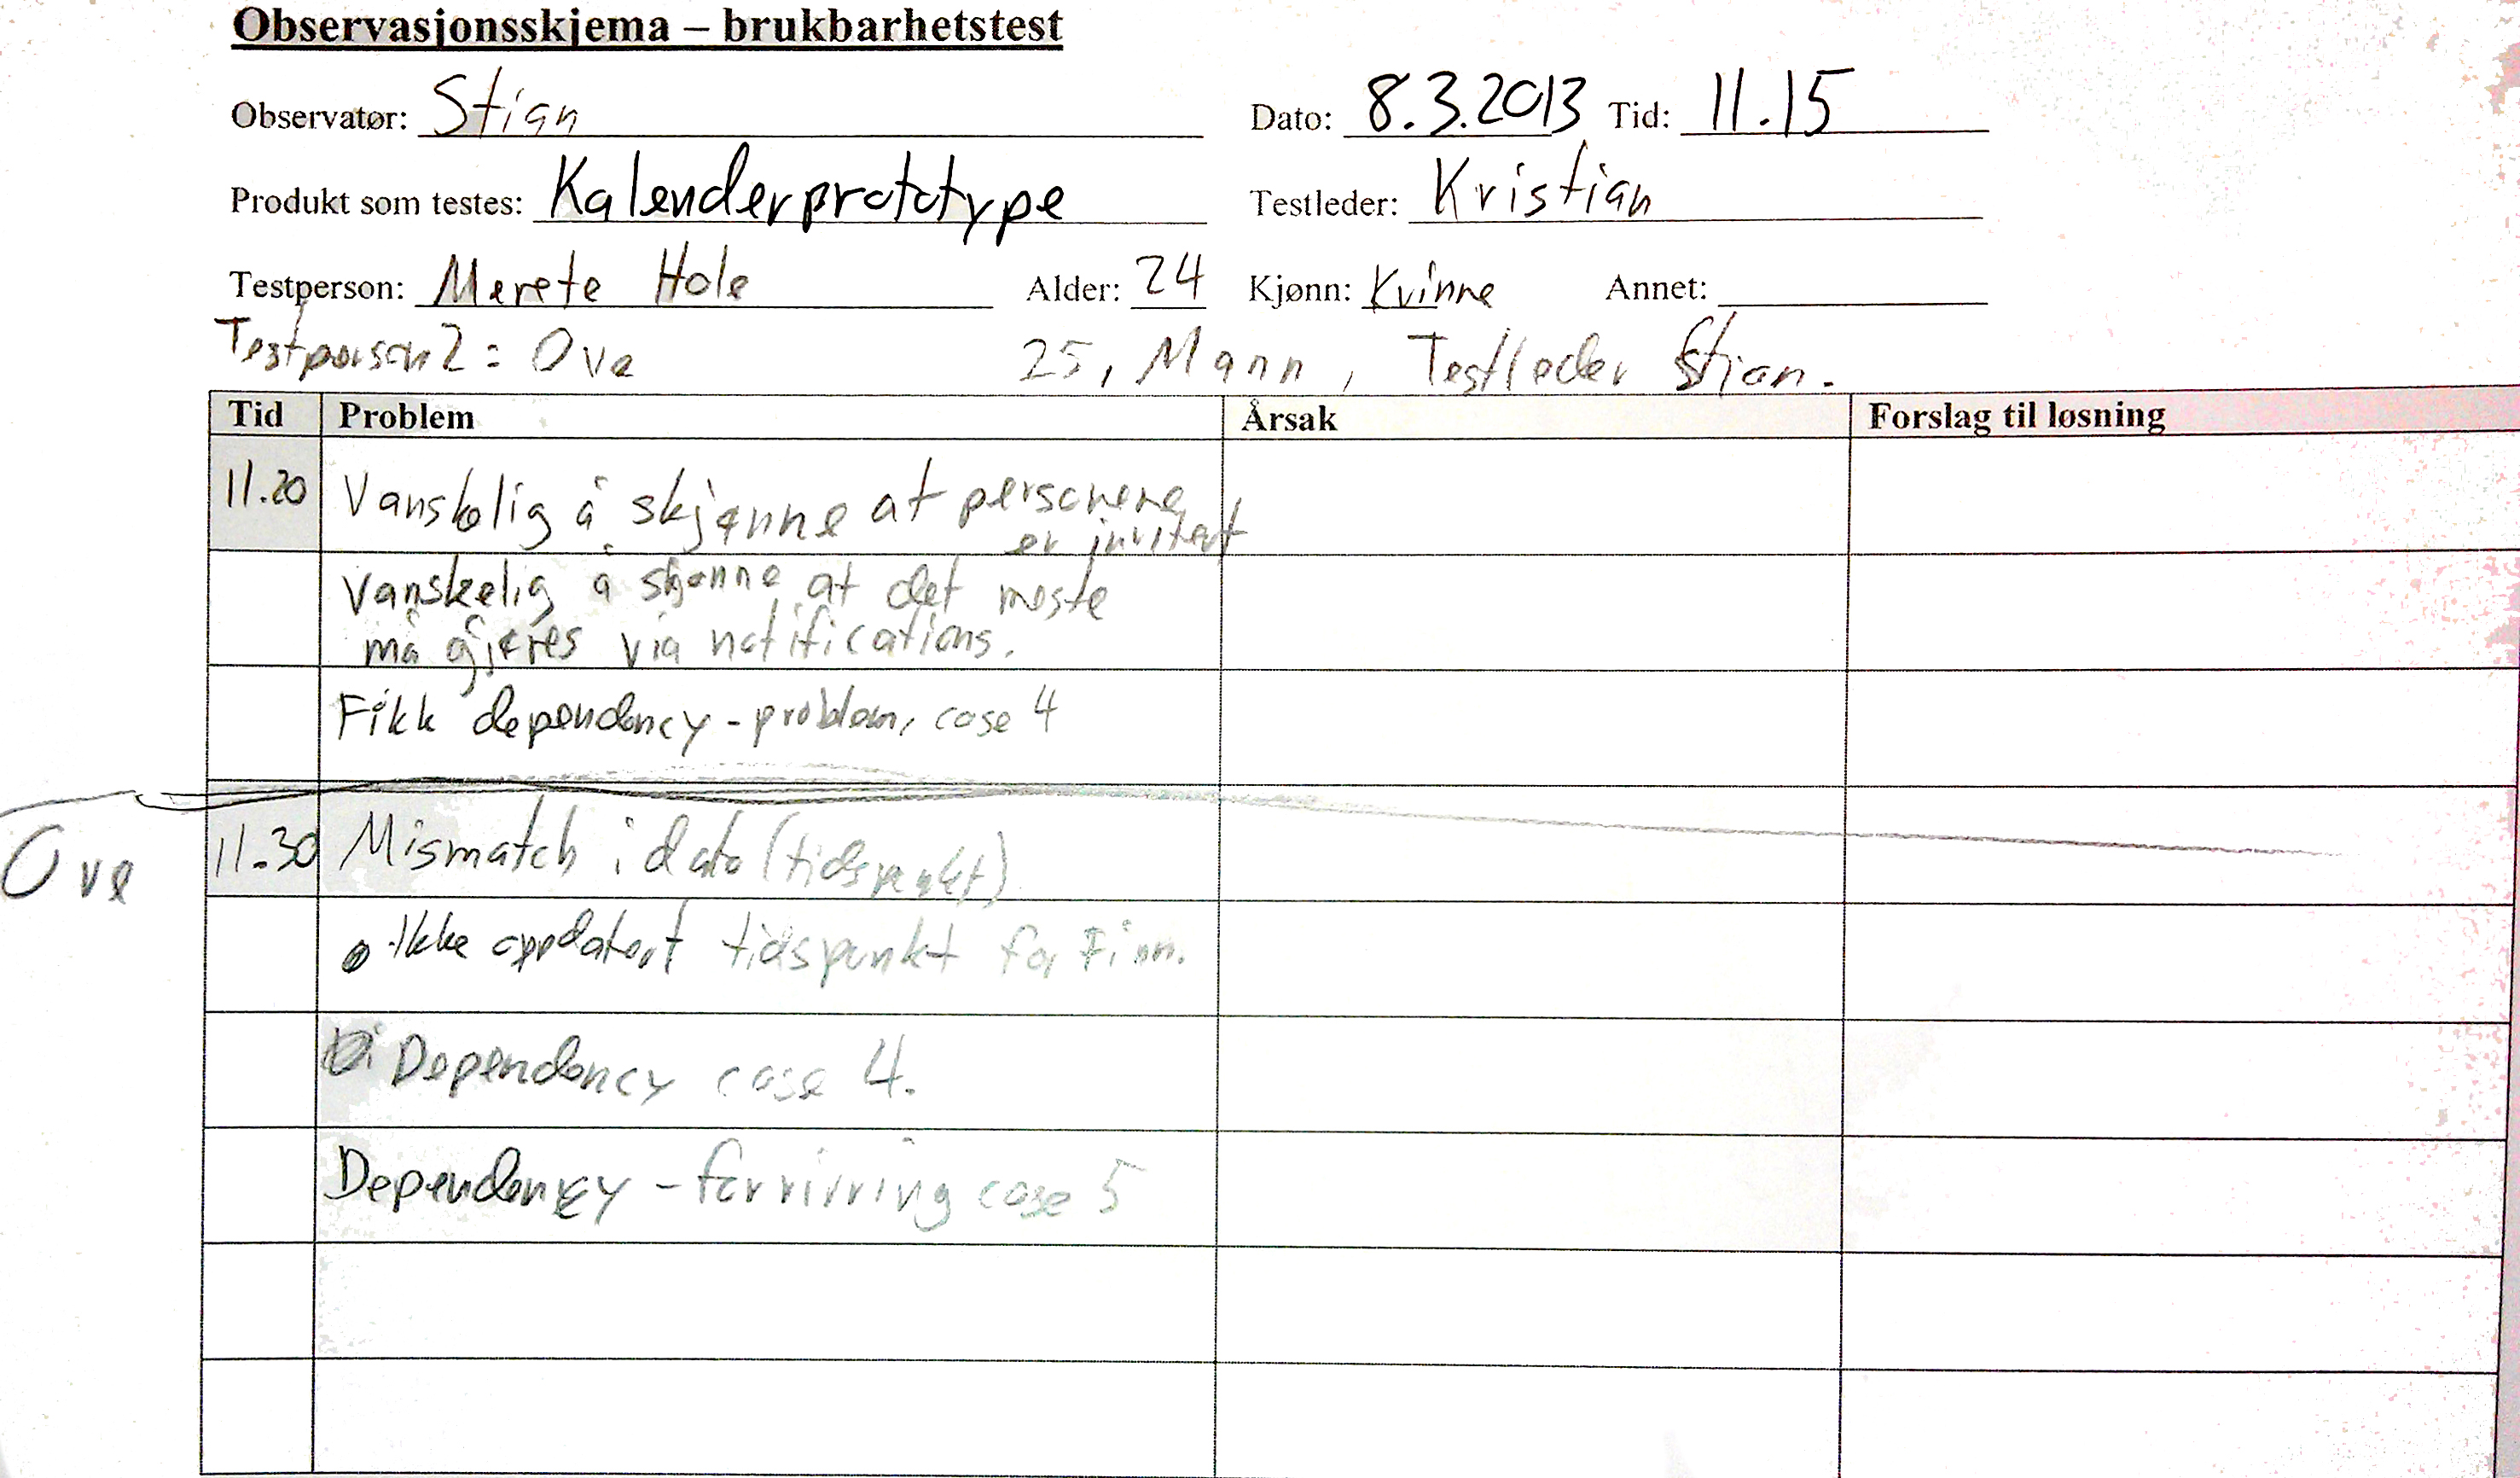
\includegraphics[width=160mm]{images/observasjon.jpg}
\caption{Observasjon}
\label{overflow}
\end{figure}

\begin{figure}[mer]
\centering
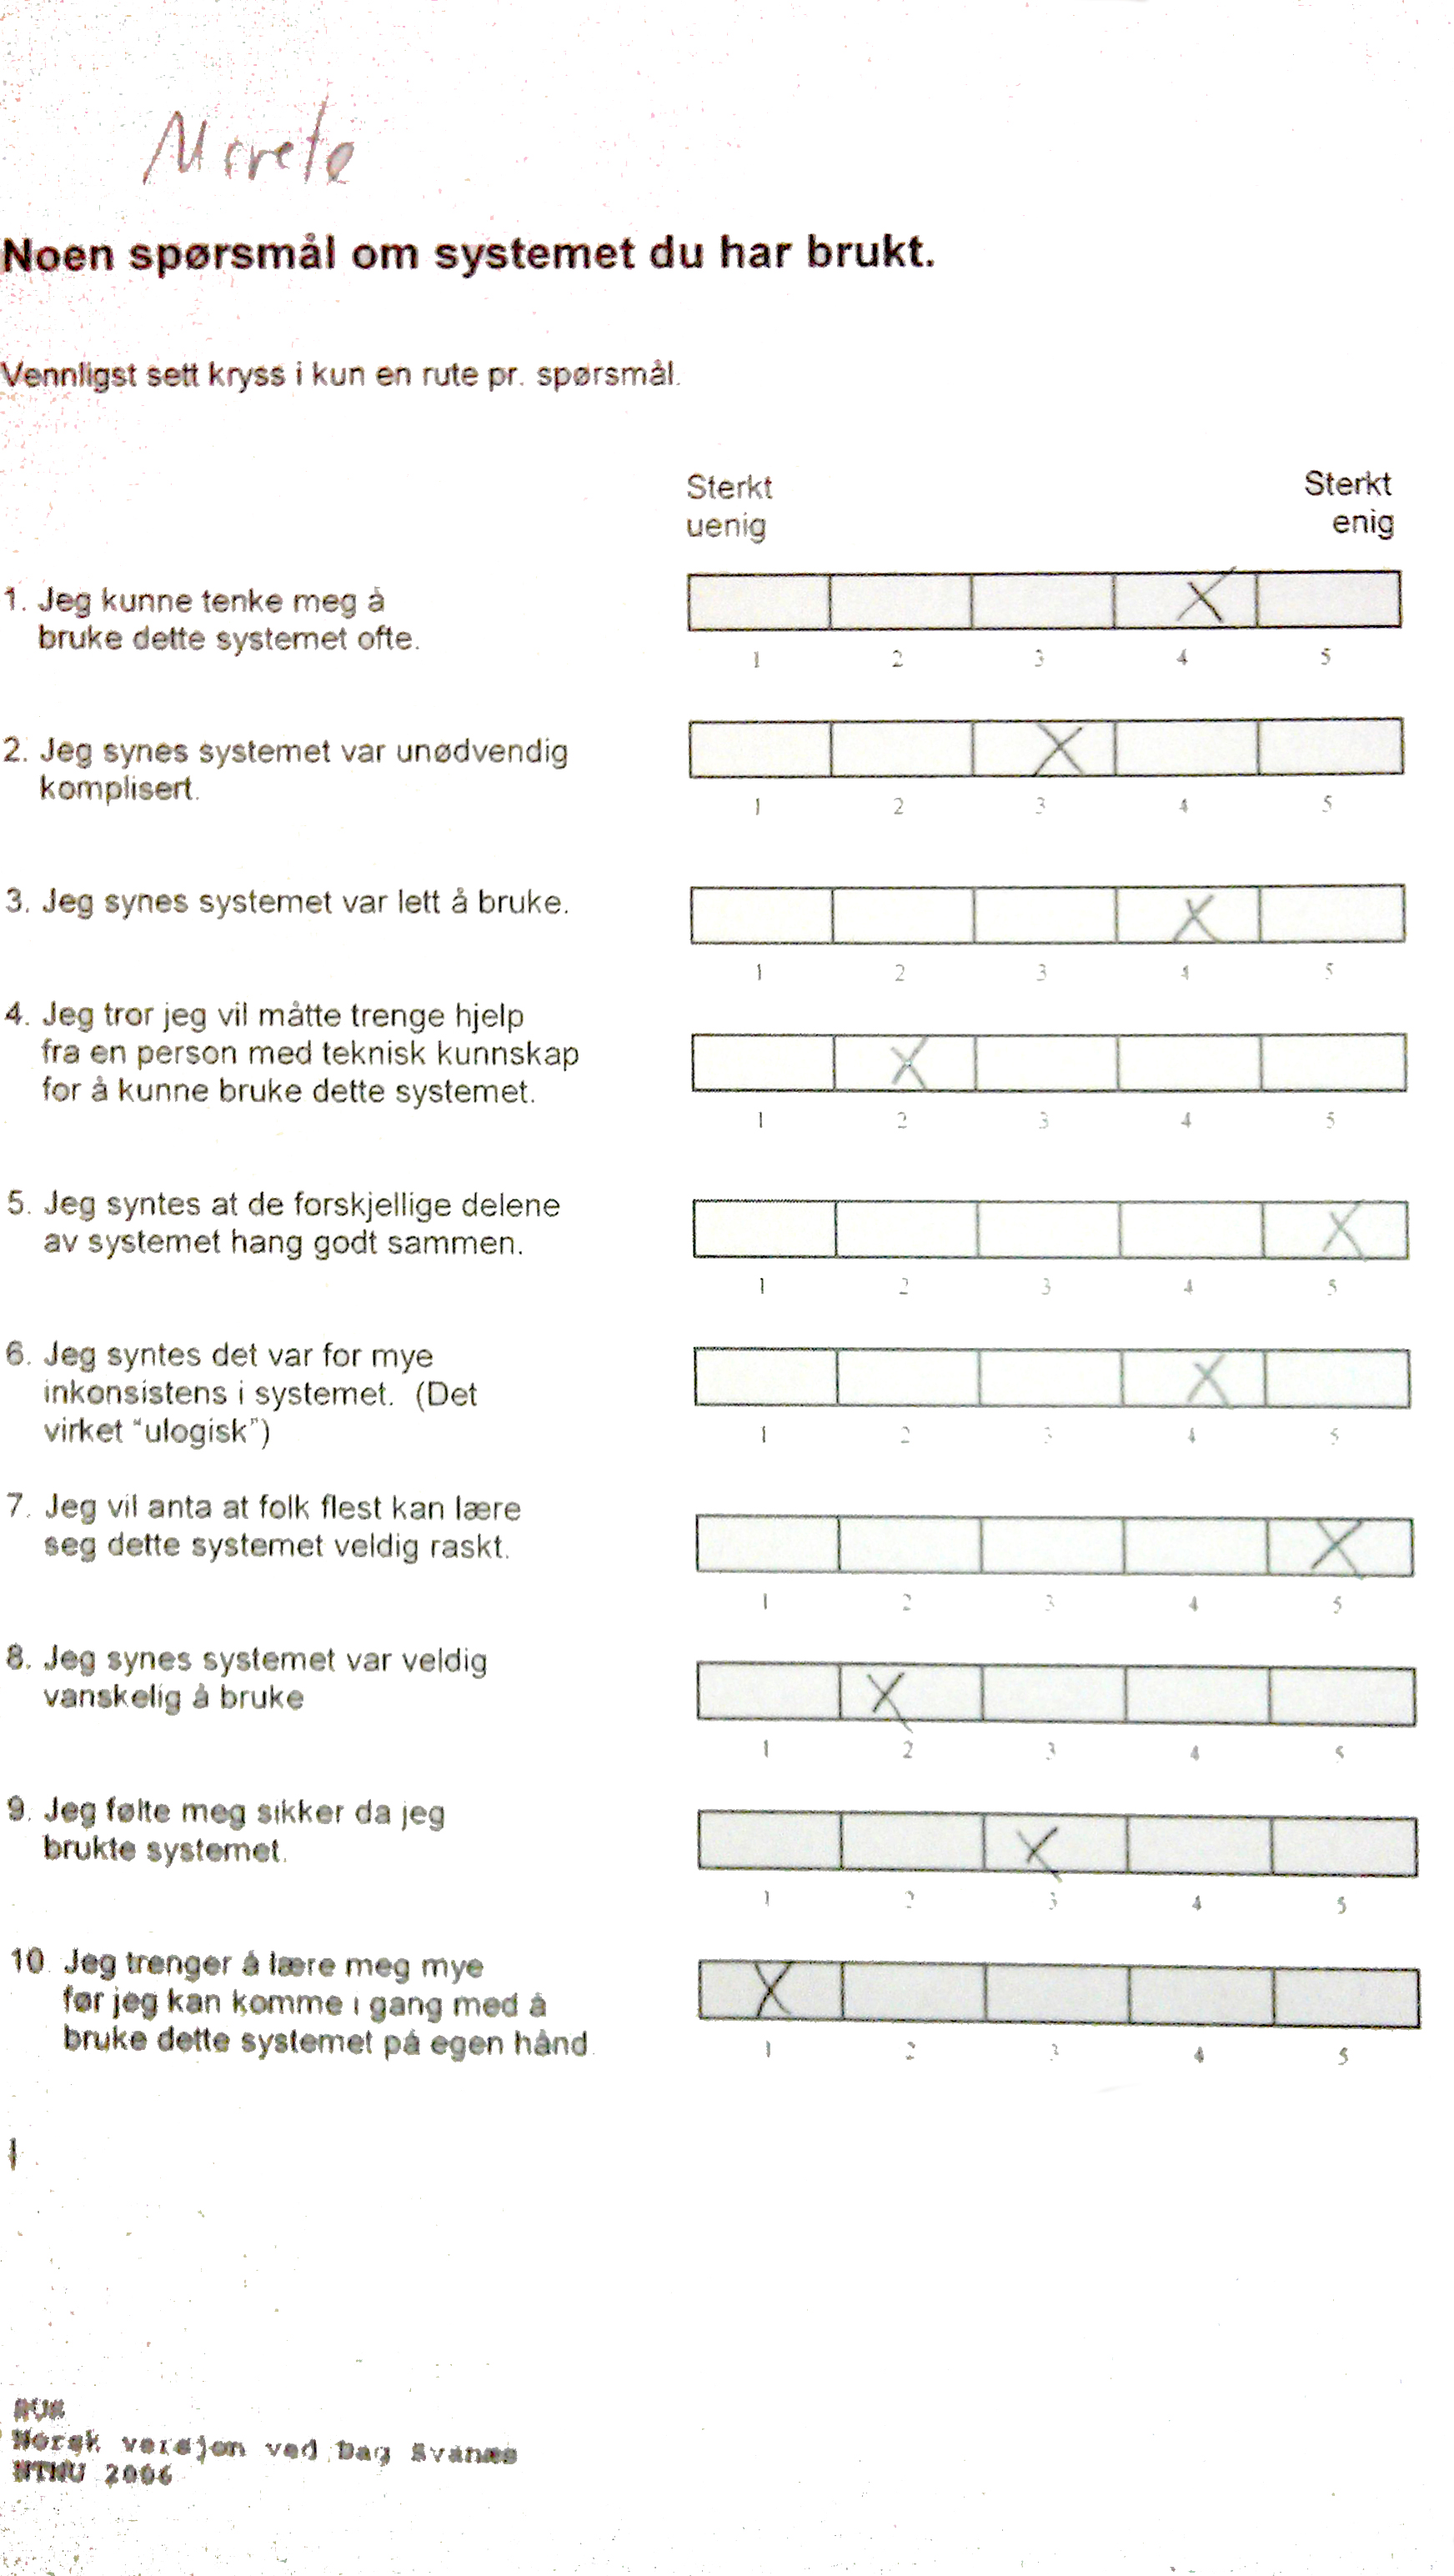
\includegraphics[width=140mm]{images/tilbakemelding_merete.jpg}
\caption{Tilbakemelding fra Merete}
\label{overflow}
\end{figure}

\begin{figure}[ove]
\centering
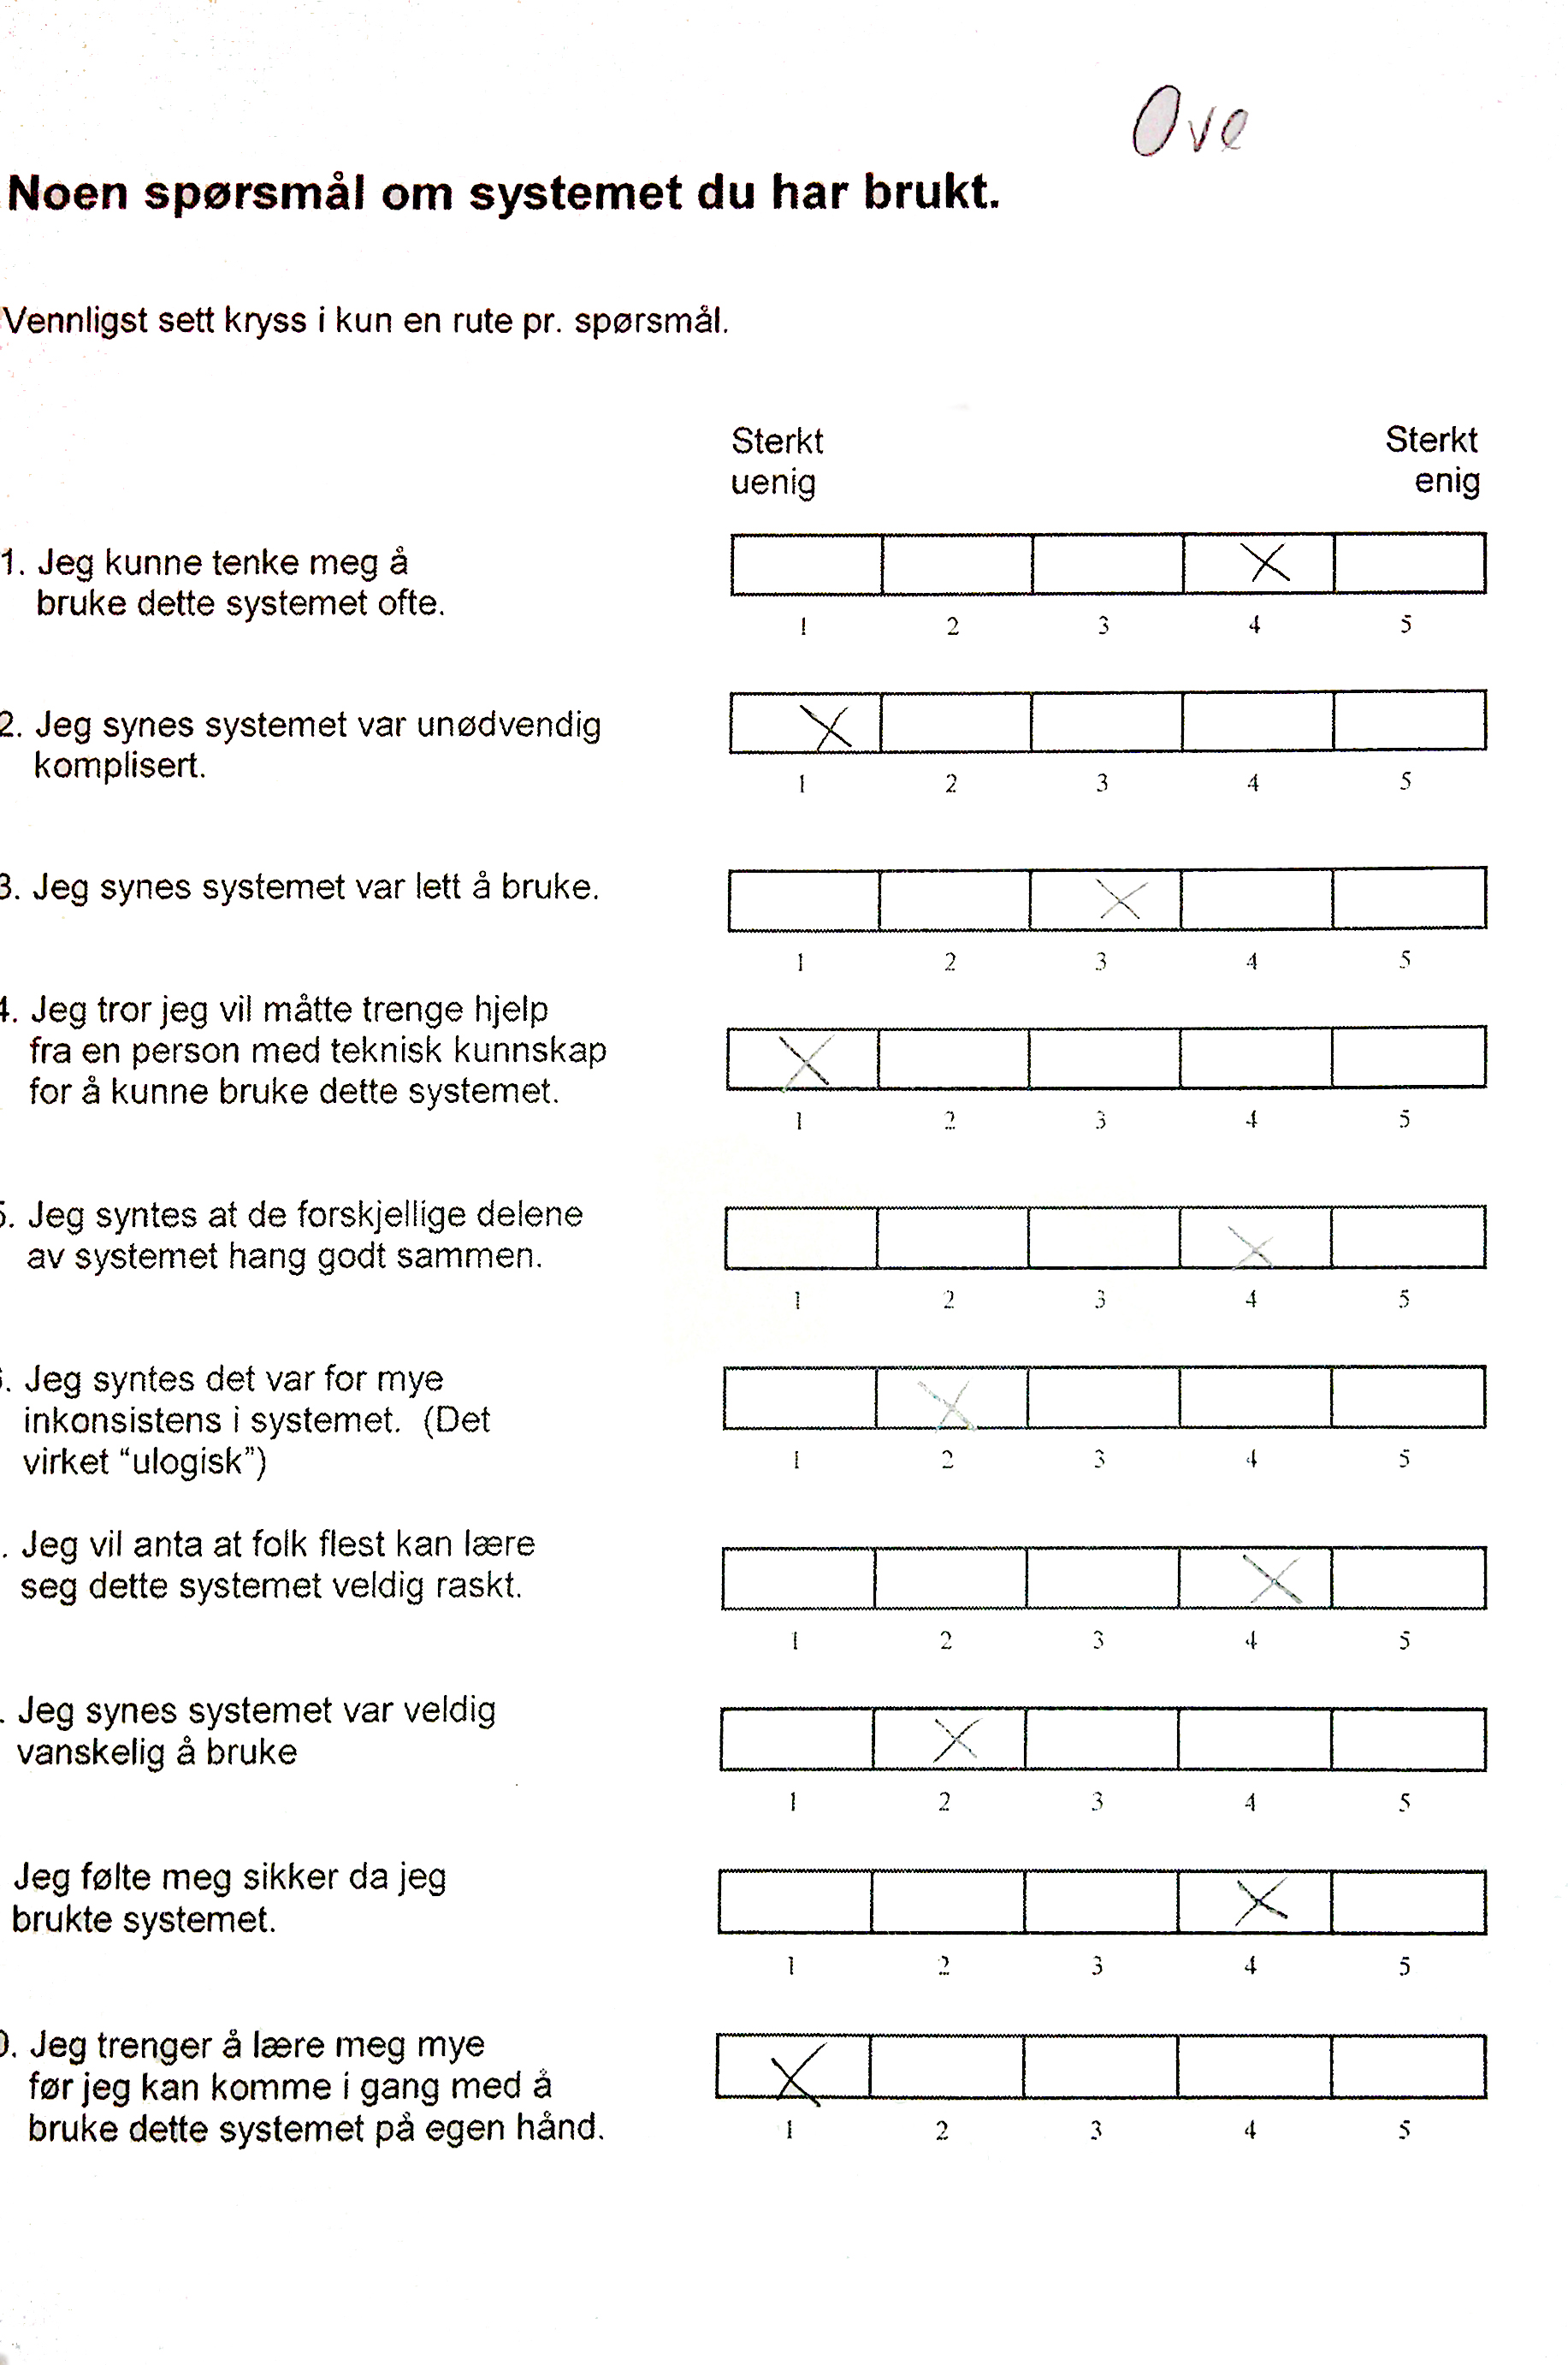
\includegraphics[width=140mm]{images/tilbakemelding_ove.jpg}
\caption{Tibakemelding fra Ove}
\label{overflow}
\end{figure}
